%   ##
%
%   Band VIII, 3 N.~??A10.3
%   Signatur/Tex-Datei: LH_35_09_15_010-011
%   RK-Nr. 41152 [Teil 3]
%   Überschrift: Tentaminum de chordarum tensione scheda tertia
%   Datierung: 1680.12.10
%   WZ: (keins)
%.  SZ: (keins)
%.  Bilddateien (PDF): LH_35_09_15_010-011_d (insgesamt eins)
%
%
\begin{ledgroupsized}[r]{120mm}
\footnotesize
\pstart
\noindent\textbf{Überlieferung:}
\pend
\end{ledgroupsized}
\begin{ledgroupsized}[r]{114mm}
\footnotesize
\pstart \parindent -6mm
\makebox[6mm][l]{\textit{L}}%
Aufzeichnung: LH XXXV 9, 15 Bl. 10\textendash11.
Ein Bogen 4\textsuperscript{o}.
Vier einspaltig beschriebene Seiten.
% Der Text von N.~??A10\textsubscript{3} wird in N.~??A10\textsubscript{4} fortgesetzt.
% Kein Wasserzeichen.
\pend
\end{ledgroupsized}
%
%
\vspace{4mm}% Vorläufig geändert 
%
%
\count\Bfootins=1000
\count\Afootins=1000
\count\Cfootins=1000
%
%
\pstart%
\normalsize%
\noindent%
%
\lbrack10~r\textsuperscript{o}\rbrack\ % Blatt 10r
%
\pend%
%
% Überschrift
\pstart%
\centering%
Tentaminum de Chordarum Tensione Scheda 3tia 10 Xb. 1680.%
\protect\index{Sachverzeichnis}{tentamen}%
\protect\index{Sachverzeichnis}{tensio chordae}%
\protect\index{Sachverzeichnis}{scheda}
\pend%
 \vspace{0.5em}%
%
%
%  \vspace{1.0em}%
%%  \newpage%  !!!!! Rein vorläufig !!!!!
%  \centerline{\includegraphics[width=0.70\textwidth]{gesamttex/edit_VIII,3/images/LH_35_09_15_010-011_d.pdf}}%\\
%  \vspace{0.5em}
%  \centerline{\lbrack\textit{Fig.~1}\rbrack}\label{LH_35_09_15_010r_fig.1}%
%%  \newpage%  !!!!! Rein vorläufig !!!!!
%  %\vspace*{1.5em}%
%%
%%
\pstart%
\noindent%
Sit chorda $QAB,$\protect\index{Sachverzeichnis}{chorda tensa}
cujus longitudo $AB,$\protect\index{Sachverzeichnis}{longitudo chordae}
crassities $AQ,$\protect\index{Sachverzeichnis}{crassities chordae}
quae pondere $E$\protect\index{Sachverzeichnis}{pondus sustentans}
\edtext{tensa sustentetur.
Aucto jam}{%
\lemma{tensa}\Bfootnote{%
\textit{(1)}~teneatur
\textit{(2)}~sustentetur.
\textit{(a)}~Sit ite
\textit{(b)}~Aucto jam%
~\textit{L}}}
pondere $E,$
ut inde fiat pondus $N,$\protect\index{Sachverzeichnis}{pondus sustentans}
extendatur ex longitudine $AB$ in longitudinem $LM,$\protect\index{Sachverzeichnis}{longitudo chordae}
et
\edtext{ex crassitie $AQ$ in crassitiem $LP,$\protect\index{Sachverzeichnis}{crassities chordae}
longitudines erunt inter se\protect\index{Sachverzeichnis}{longitudo chordae}
ut pondera,\protect\index{Sachverzeichnis}{pondus tendens}
et in reciproca ratione crassitierum\protect\index{Sachverzeichnis}{crassities chordae} duplicata,}{%
\lemma{ex}\Bfootnote{% \hspace*{-0,5mm}
\textit{(1)}~longitudine $A$
\textit{(2)}~crassitie $AQ$ in crassitiem $LP,$
\textit{(a)}~sintque
\textit{(b)}~longitudines
\textit{(aa)}~crassitiebus erunt reciproce proportionales, seu erunt
\textit{(bb)}~erunt inter \lbrack...\rbrack\ crassitierum duplicata,%
~\textit{L}}}
%seu erit:
$\displaystyle AB : \overline{LP}\,\boxed{\scriptstyle{2}} : E \,\squaredots\, LM : \overline{AQ}\,\boxed{\scriptstyle{2}} : N.$
\edtext{Ut patet
\edtext{ex superioribus.}{%
\lemma{ex superioribus}\Cfootnote{%
Siehe N.~8\textsubscript{2}, S.~\refpassage{LH_35_09_15_008v_siluaekg-1}{LH_35_09_15_009r_siluaekg-2}.}}% 
% N.~??A10\textsubscript{1}, S.~\refpassage{LH_35_09_15_007v_schd3.1-1}{LH_35_09_15_007v_schd3.1-2}; N.~??A10\textsubscript{2}, S.~\refpassage{LH_35_09_15_008v_vrws-1-1}{LH_35_09_15_008v_vrws-1-2}
}{%
\lemma{Ut}\Bfootnote{%
\hspace{-0,5mm}patet ex superioribus.
\textit{erg.~L}}}%
\edtext{}{%
\lemma{\textit{Am Rand, gestr.}}\Afootnote{%
\footnotesize{%
NB non debuisset sumi $ABS$ in extremo, sed in medio,
ut similis esset ipsi $RLP.$% 
\vspace{-1,4em}
}}}
% \pend%
%
% \pstart%
Manifestum
\edtext{est etiam ex
\edtext{superius assumtis}{\lemma{ex superius assumtis}\Cfootnote{%
Siehe N.~8\textsubscript{2}, S.~\refpassage{LH_35_09_15_009v_schd3.2-1}{LH_35_09_15_009v_schd3.2-2} (gestrichener Text).}}%
}{%
\lemma{est}\Bfootnote{%
\hspace{-0,5mm}\textbar~etiam \textit{erg.}~\textbar\ ex
\textit{(1)}~supra demonstratis
\textit{(2)}~superius assumtis%
~\textit{L}}}
%
chordam\protect\index{Sachverzeichnis}{chorda tensa}
\edtext{tensam $BAQ$}{%
\lemma{tensam}\Bfootnote{%
\textit{(1)}~$AB$
\textit{(2)}~$BAQ$%
~\textit{L}}}
et chordam tensam $MLP,$
cum sint diversi status\protect\index{Sachverzeichnis}{status chordae}
ejusdem chordae tensae\protect\index{Sachverzeichnis}{chorda tensa}
cujus status naturalis\protect\index{Sachverzeichnis}{status naturalis} sit verbi gratia $TAQ,$
ad eum reduci eodem tempore.
Sed si prius ambae pulsentur seu ulterius tendantur,
atque inde omnino dimittantur usque ad statum naturalem,\protect\index{Sachverzeichnis}{status naturalis}
cum tempora a pulsatione\protect\index{Sachverzeichnis}{pulsatio chordae}
seu a secunda tensione ad primam tensionem\protect\index{Sachverzeichnis}{tensio chordae}
non possunt esse aequalia\protect\index{Sachverzeichnis}{tempus restitutionis}
(\phantom)\hspace*{-1.2mm}%
quia
\edtext{constat esse}{%
\lemma{constat}\Bfootnote{%
\hspace{-0,5mm}esse \textit{erg.~L}}}
magisque minusque tensarum\protect\index{Sachverzeichnis}{chorda tensa}
inaequales post pulsationem\protect\index{Sachverzeichnis}{pulsatio chordae}
restitutiones\protect\index{Sachverzeichnis}{restitutio chordae}
ad primam tensionem,\protect\index{Sachverzeichnis}{tensio chordae}%
\phantom(\hspace*{-1.2mm})
\edtext{ideoque sequi videtur}{%
\lemma{ideoque}\Bfootnote{%
\textit{(1)}~necesse est
\textit{(2)}~sequi videtur%
~\textit{L}}}
chordam $MLP$\protect\index{Sachverzeichnis}{chorda pulsata} pulsatam
% \edtext{}{%
% \lemma{pulsatam}\Bfootnote{%
% \textit{(1)}~quia
% \textit{(2)}~quia%
% ~\textit{L}}}
quia a secunda tensione ad\protect\index{Sachverzeichnis}{tensio chordae}
\edtext{primam $MLP$ celerius}{%
\lemma{primam}\Bfootnote{%
\hspace{-0,5mm}\textbar~$MLP$ \textit{erg.}~%
\textbar\ celerius%
~\textit{L}}}
restituitur,
\edtext{quam $BAQ$}{%
\lemma{quam}\Bfootnote{%
\hspace{-0,5mm}$BAQ$ \textit{erg.~L}}}
a prima
\edtext{tensione\protect\index{Sachverzeichnis}{tensio chordae}}{%
\lemma{tensione}\Bfootnote{\textit{erg.~L}}}%
\lbrack,\rbrack\
%\newpage
%  \centerline{\includegraphics[width=0.66\textwidth]{gesamttex/edit_VIII,3/images/LH_35_09_15_010-011_d.pdf}}%\\
%  \vspace{-0.5em}
%  \centerline{\lbrack\textit{Fig.~1}\rbrack}\label{LH_35_09_15_010r_fig.1}%
%%  \newpage%  !!!!! Rein vorläufig !!!!!
%  \vspace{1.0em}%
 postea tardius restitui ad statum naturalem\protect\index{Sachverzeichnis}{status naturalis}\edlabel{KZeitz7}%
\edtext{}%
{{\xxref{KZeitz7}{KZeitz8}}%
{\lemma{$TAQ$}\Bfootnote{%
\textit{(1)}~. Sed \textbar~jam \textit{erg.}~\textbar\ video in quo error
\textit{(2)}~. Quod non capio quomodo sit possibile. Sed error. Nempe non
\textit{(a)}~possunt distingui
\textit{(b)}~potest distingui
\textit{(c)}~vera est inaequalitas tunc cum di
\textit{(3)}~, contra hypothesin. \lbrack...\rbrack\ distincta esse
\textit{(a)}~a 
\textit{(aa)}~secund
\textit{(bb)}~pri
\textit{(b)}~a restitutione \lbrack...\rbrack\ ut sit
\textit{(aa)}~inaequalitas
\textit{(bb)}~inaequalitas in illis,%
~\textit{L}}}}%
$TAQ,$ contra hypothesin.\protect\index{Sachverzeichnis}{hypothesis}
Sed error\protect\index{Sachverzeichnis}{error} subest in
\pend
\newpage
  \centerline{\includegraphics[width=0.66\textwidth]{gesamttex/edit_VIII,3/images/LH_35_09_15_010-011_d.pdf}}%\\
  \vspace{-0.5em}
  \centerline{\lbrack\textit{Fig.~1}\rbrack}\label{LH_35_09_15_010r_fig.1}%
  \vspace{1.5em}%
 \count\Bfootins=1100
\count\Afootins=1000
\count\Cfootins=1100
\pstart
\noindent tali ratiocinatione.\protect\index{Sachverzeichnis}{ratiocinatio}
Nam Restitutio\protect\index{Sachverzeichnis}{restitutio chordae}
a secunda tensione ad primam\protect\index{Sachverzeichnis}{tensio chordae}
debet distincta esse a restitutione\protect\index{Sachverzeichnis}{restitutio chordae}
a prima ad naturalem,\protect\index{Sachverzeichnis}{tensio naturalis}
ut sit inaequalitas in illis,\edlabel{KZeitz8}
seu
\edtext{sub finem pulsationis\protect\index{Sachverzeichnis}{pulsatio chordae}}{%
\lemma{sub}\Bfootnote{%
\textit{(1)}~initium
\textit{(a)}~dimi
\textit{(b)}~dimissionis
\textit{(2)}~finem pulsationis%
~\textit{L}}}
non debet esse omnimoda
\edtext{dimissio,\protect\index{Sachverzeichnis}{dimissio chordae omnimoda}
ut locum habeat hypothesis\protect\index{Sachverzeichnis}{hypothesis} praesens
seu ut inaequales sint restitutiones a prima tensione ad secundam.
Atque ita sublata est haec difficultas.\protect\index{Sachverzeichnis}{difficultas}}{%
\lemma{dimissio,}\Bfootnote{%
\textit{(1)}~ut inaequalis sit restitutio a
\textit{(2)}~ut locum habeat hypothesis praesens
\textit{(a)}~et
\textit{(b)}~seu ut \lbrack...\rbrack\ restitutiones a
\textit{(aa)}~prima
\textit{(bb)}~secu
\textit{(cc)}~prima tensione ad secundam.
\textit{(aaa)}~Alioqui enim aequales sunt restitutiones.
\textit{(bbb)}~Atque ita \lbrack...\rbrack\ haec difficultas.%
~\textit{L}}}
\edtext{Chorda enim pulsata\protect\index{Sachverzeichnis}{chorda pulsata}
seu adducta a prima tensione ad novam,\protect\index{Sachverzeichnis}{tensio chordae}
atque dimissa\protect\index{Sachverzeichnis}{chorda dimissa}
non est omnimoda dimissio,\protect\index{Sachverzeichnis}{dimissio chordae omnimoda}
sed superest prior tensio.\protect\index{Sachverzeichnis}{tensio chordae}}{%
\lemma{Chorda}\Bfootnote{%
\hspace{-0,5mm}enim pulsata
\textbar~seu adducta \textit{erg.}~%
\textbar\ a prima \lbrack...\rbrack\ prior tensio.
\textit{erg.~L}}}
\pend%
\vspace{0.5em}
%
\pstart%
\noindent%
\lbrack\textit{Nachfolgend kleingedruckter Text in L gestrichen:}\rbrack\
\pend%
\vspace{0.5em}
%
\footnotesize%
\pstart%
Sit chorda $BAS$ similis chordae $MLP,$\protect\index{Sachverzeichnis}{chorda tensa}
id est ejusdem materiae\protect\index{Sachverzeichnis}{materia chordae}
et crassitiei\protect\index{Sachverzeichnis}{crassities chordae}\lbrack,\rbrack\
et sumatur in chorda $MLP$
\edtext{ipsa $RLP,$}{%
\lemma{ipsa}\Bfootnote{%
\textit{(1)}~$ARP$
\textit{(2)}~$RLP,$%
~\textit{L}}}
aequalis et similis ipsi $BAS,$
differentia erit in solis
\edtext{tensionibus.\protect\index{Sachverzeichnis}{tensio chordae}
\edtext{Ex supradictis}{%
\lemma{Ex supradictis}\Cfootnote{%
Siehe N.~8\textsubscript{2}, S.~\refpassage{LH_35_09_15_009v_utlong-1}{LH_35_09_15_009v_utlong-2}.}}
\lbrack manifestum est\rbrack}{%
\lemma{tensionibus.}\Bfootnote{%
\textit{(1)}~Manifestum est
\textit{(2)}~Ex supradictis
\textbar~manifestum est \textit{erg. Hrsg.}~\textbar%
~\textit{L}}}
%
tempus restitutionis\protect\index{Sachverzeichnis}{tempus restitutionis} ipsius $RLP$
esse ad tempus restitutionis\protect\index{Sachverzeichnis}{tempus restitutionis} ipsius $MLP,$
\edtext{ut $RL$ ad $ML.$}{%
\lemma{ut}\Bfootnote{%
\textit{(1)}~$ER$ ad
\textit{(2)}~$RL$ ad $ML.$%
~\textit{L}}}
%
\edtext{Intelligo restitutiones praesectarum\protect\index{Sachverzeichnis}{restitutio chordae}
a tensione 2da ad primam.\protect\index{Sachverzeichnis}{tensio chordae}}{%
{\lemma{Intelligo}\Bfootnote{%
\hspace{-0,5mm}restitutiones praesectarum
\textit{(1)}~ad pri
\textit{(2)}~a tensione 2da ad primam
\textbar~praesectarum \textit{gestr.}~%
\textbar~. \textit{erg.~L}}}
{\lemma{Intelligo \lbrack...\rbrack\ primam}\Cfootnote{%
Siehe N.~8\textsubscript{2}, S.~\refpassage{LH_35_09_15_009v_restprsct-1}{LH_35_09_15_009v_restprsct-2}.}}}
\newline%
\count\Bfootins=1000
\count\Afootins=1000
\count\Cfootins=1000
\indent%
Si%
\edlabel{LH_35_09_15_010v_scd3.6-1}
jam duarum chordarum aequalium et similium
\edtext{restitutiones\protect\index{Sachverzeichnis}{restitutio chordae} sint}{%
\lemma{restitutiones}\Bfootnote{%
\textit{(1)}~sint
\textit{(2)}~ad primam tensionem sint
\textit{(3)}~sint%
~\textit{L}}}
ut tensiones\protect\index{Sachverzeichnis}{tensio chordae}
seu ut pondera\protect\index{Sachverzeichnis}{pondus appensum}
appensa\lbrack,\rbrack\ erit
% \edtext{}{%
% \lemma{appensa}\Bfootnote{%
% \textit{(1)}~et rit
% \textit{(2)}~erit%
% ~\textit{L}}}
\edtext{tempus\protect\index{Sachverzeichnis}{tempus restitutionis} seu}{%
\lemma{tempus}\Bfootnote{%
\hspace{-0,5mm}seu \textit{erg.~L}}}
restitutio
\edtext{chordae\protect\index{Sachverzeichnis}{restitutio chordae} $BAS$ seu
(\phantom)\hspace*{-1.2mm}%
quia crassities\protect\index{Sachverzeichnis}{crassities chordae}
non variat tempus\protect\index{Sachverzeichnis}{tempus restitutionis}%
\phantom(\hspace*{-1.2mm})
chordae $BAQ$}{%  a $BAQ$
\lemma{chordae}\Bfootnote{%
\textit{(1)}~$BAS$
\textit{(2)}~$BAQ$
\textit{(3)}~$BAS$ seu \lbrack...\rbrack\ chordae $BAQ$%
~\textit{L}}}
%
ad restitutionem\protect\index{Sachverzeichnis}{restitutio chordae}
\edtext{chordae $RPL,$ reciproce ut tensio\protect\index{Sachverzeichnis}{tensio chordae}
ipsius $BAQ$ ad tensionem ipsius $RLP$ seu $MLP$\protect\index{Sachverzeichnis}{tensio chordae}\lbrack;\rbrack\
seu Rest. $BAQ$ : Rest. $RLP\ \squaredots $ Tens. $MLP$ : Tens. $BAQ\, \squaredots\, N : E\, \squaredots\, ML : BA \, \squaredots\, ML : RL.\ $
Rest. $RLP$~: Rest. $MLP\, \squaredots\, RL : ML.\ $
Ergo Rest. $BAQ$ aequ. Rest. $MLP$.\protect\index{Sachverzeichnis}{restitutio chordae}
Quod est absurdum.}{%
\lemma{chordae}\Bfootnote{%
\hspace{-0,5mm}$RPL,$
\textit{(1)}~ut
\textit{(a)}~pondus
\textit{(b)}~pondus $N$ ad
\textit{(aa)}~pondus
\textit{(bb)}~ponderis $N$ partem quae sit ad ipsam ut $RL$ ad $ML$
\textit{(aaa)}~seu Rest. $RLP$ : Rest.
\textit{(bbb)}~seu Rest. $BAQ$ : Rest. $RLP\ \squaredots$ ut $\displaystyle\frac{LR}{ML}N.$
\textit{(aaaa)}~Et Rest. $RLP$ : Rest. $MLP\ \squaredots$
\textit{(bbbb)}~Jam aliunde Rest. $RLP$ : Rest. $MRL$
\textit{(2)}~reciproce ut tensio \lbrack...\rbrack\ Quod est absurdum.%
~\textit{L}}}
%
\lbrack10~v\textsuperscript{o}\rbrack% Blatt 10v
%
\pend%
\count\Bfootins=1000
\count\Afootins=1000
\count\Cfootins=1000
%
% \footnotesize
\pstart%
Haec sane ratiocinatio\protect\index{Sachverzeichnis}{ratiocinatio}
\edtext{mirifice turbare videtur,}{%
\lemma{mirifice}\Bfootnote{%
\textit{(1)}~turbat,
\textit{(2)}~turbare videtur,%
~\textit{L}}}
cum enim certum sit chordas $ABQ$ et $MLP$\protect\index{Sachverzeichnis}{chorda tensa}
restitui diversis temporibus,\protect\index{Sachverzeichnis}{tempus restitutionis}
nempe magis tensam $MLP$ celerius\lbrack,\rbrack\
\edtext{adeoque absurda sit conclusio;\protect\index{Sachverzeichnis}{conclusio absurda}}{%
\lemma{adeoque}\Bfootnote{%
\hspace{-0,5mm}absurda sit conclusio \textit{erg.~L}}}
necesse est vel aliquid praecedentium esse falsum,
vel id quod hic unicum assumsimus
\edtext{in praesenti ratiocinatione,\protect\index{Sachverzeichnis}{ratiocinatio}}{%
\lemma{in}\Bfootnote{%
\hspace{-0,5mm}praesenti ratiocinatione \textit{erg.~L}}}
duarum chordarum sola tensione\protect\index{Sachverzeichnis}{tensio chordae}
differentium restitutiones\protect\index{Sachverzeichnis}{restitutio chordae}
seu restituendi tempora\protect\index{Sachverzeichnis}{tempus restituendi}
esse ut
\edtext{tensiones reciproce,\protect\index{Sachverzeichnis}{tensio chordae}
seu restituendi celeritates\protect\index{Sachverzeichnis}{celeritas restituendi}}{%
\lemma{tensiones}\Bfootnote{%
\textit{(1)}~celer
\textit{(2)}~reciproce, seu restituendi celeritates%
~\textit{L}}}
esse ut
\edtext{tensiones.\protect\index{Sachverzeichnis}{tensio chordae}
Itaque positis praecedentibus concludere possumus hoc esse falsum.%
\edlabel{LH_35_09_15_010v_scd3.6-2}
Imo ut lucremur aliquam veritatem positivam\protect\index{Sachverzeichnis}{veritas positiva}
investigemus quid oriatur ratione restitutionum\protect\index{Sachverzeichnis}{restitutio chordae}
inter chordas aequales et similes inaequaliter tensas\protect\index{Sachverzeichnis}{chorda tensa}
assumta utcunque.
\newline%
\indent%
\textso{Ejusdem chordae}}{%
\lemma{tensiones.}\Bfootnote{%
\textit{(1)}~Imo hoc concludere possumus:
\textbar~positis praecedentibus, \textit{erg.}~\textbar\
\textit{(a)}~duarum chordarum diversarum
\textit{(b)}~diversarum chordarum
\textit{(c)}~quod \textso{duarum diversarum}
\textit{(2)}~Itaque
\textit{(a)}~conlud
\textit{(b)}~positis praecedentibus \lbrack...\rbrack\ investigemus quid
\textit{(aa)}~ass
\textit{(bb)}~oriatur
\textit{(aaa)}~assumta
\textit{(bbb)}~ratione restitutionum inter chordas
\textit{(aaaa)}~aeque tensas
\textit{(bbbb)}~aequales et \lbrack...\rbrack\ \textso{Ejusdem chordae}%
~\textit{L}}}%
\textso{ tensionum }\protect\index{Sachverzeichnis}{tensio chordae}%
\edtext{\textso{restitutiones sunt inter}}{%
\lemma{\textso{restitutiones}}\Bfootnote{%
\textit{(1)}~\textso{inter}
\textit{(2)}~\textso{sunt inter}%
~\textit{L}}}%
\textso{ se ut restitutiones duarum chordarum\protect\index{Sachverzeichnis}{restitutio chordae}}%
\textso{ aequalium et similium
easdem diversas tensiones habentium.}
Quae propositio\protect\index{Sachverzeichnis}{propositio} si falsa est,
\edtext{necesse est aliquam}{%
\lemma{necesse}\Bfootnote{%
\hspace{-0,5mm}est
\textit{(1)}~aliquod
\textit{(2)}~aliquam%
~\textit{L}}}
ex superioribus nostris hypothesibus\protect\index{Sachverzeichnis}{hypothesis}
\edtext{assumtis esse falsam.
Iis autem positis}{%
\lemma{assumtis}\Bfootnote{%
\textit{(1)}~corrigendam esse.
\textit{(a)}~Nulla
\textit{(aa)}~sane
\textit{(bb)}~sane
\textit{(b)}~Quod chordae inaequa
\textit{(c)}~Quaenam autem sit corrigenda
\textit{(aa)}~corrigem
\textit{(bb)}~inquiremus, ubi sciemus an aliqua corrigenda sit
\textit{(2)}~esse falsam. Iis autem positis%
~\textit{L}}}
ipsa est demonstrata.
Demonstratio\protect\index{Sachverzeichnis}{demonstratio} autem talis erit
praecedenti nonnhil mutata:%
%
\pend%
\vspace{0.5em}%
%\newpage%
%
\normalsize%
\pstart%
Chordarum\protect\index{Sachverzeichnis}{chorda tensa}
\edtext{similium et aequalium, sed inaequaliter tensarum
$RLP$ et $BAS$\textso{ restitutiones }\protect\index{Sachverzeichnis}{restitutio chordae}%
seu restitutionum tempora\protect\index{Sachverzeichnis}{tempus restitutionis}
sunto inter se illius ut $p,$ huius ut $s.$}{%
\lemma{similium}\Bfootnote{%
\textit{(1)}~aequaliter tensarum, seu 
\textit{(2)}~et aequalium, \lbrack...\rbrack\ $RLP$ et % sed inaequaliter tensarum 
\textit{(a)}~$BAQ$
\textit{(b)}~$BAS$
\textit{(aa)}~esse ut $p$ ad $q.$
\textit{(bb)}~\textso{restitutiones}
\textit{(aaa)}~sunto inter se ut $q$ ad
\textit{(bbb)}~seu restitutionum \lbrack...\rbrack\ inter se % tempora sunto 
\textit{(aaaa)}~illa in
\textit{(bbbb)}~illius ut $p,$
\textit{(aaaaa)}~in hac
\textit{(bbbbb)}~huius ut
\textit{(aaaaa-a)}~$q$
\textit{(bbbbb-b)}~$s.$%
~\textit{L}}}
\pend%
%\newpage%
%
\pstart%
Hinc ratiocinatio\protect\index{Sachverzeichnis}{ratiocinatio}
\edtext{prodibit: % \edlabel{LH_35_09_15_010v_umbuchsdcfg-1}
% \newline%
%
% \indent%
Restit.\protect\index{Sachverzeichnis}{restitutio chordae}%
\edlabel{LH_35_09_15_010v_rtcmpst-1}
$BAS$\edlabel{LH_35_09_15_010v_umbuchsdcfg-1}}{%
\lemma{prodibit:}\Bfootnote{%
\hspace{-0,5mm}Restit.
\textit{(1)}~$BAQ$
\textit{(2)}~$BAS$%
~\textit{L}}}
: Restit. $RLP \,\squaredots\
\edtext{s : p\,$
(\phantom)\hspace*{-1.2mm}%
ex hypothesi\protect\index{Sachverzeichnis}{hypothesis}%
\phantom(\hspace*{-1.2mm}).
% \newline%
% \indent%
Jam Restit. $BAQ$ aequ. Restit. $BAS,$}{%
\lemma{$s : p$}\Bfootnote{%
\textit{(1)}~Jam Restit. $BAQ$ aequ. Restit. $BAS$
\textit{(2)}~(\phantom)\hspace*{-1.2mm}ex hypothesi\phantom(\hspace*{-1.2mm}). \lbrack...\rbrack\ Restit. $BAS,$%
~\textit{L}}}
quia crassities\protect\index{Sachverzeichnis}{crassities chordae}
non variat tempus restitutionis;\protect\index{Sachverzeichnis}{tempus restitutionis}
% \newline%
% \indent%
Ergo \makebox[1.0\textwidth][s]{Restit. $BAQ :$ Restit. $RLP \,\squaredots\ s : p.$%
\protect\index{Sachverzeichnis}{restitutio chordae}
% \newline%
% \indent%
Jam Restit. $RLP :$ Restit.\protect\index{Sachverzeichnis}{restitutio chordae}
\edlabel{KZeitz9}%
\edtext{}%
{{\xxref{KZeitz9}{KZeitz10}}%
{\lemma{$MLP \ \squaredots$}\Bfootnote{%
\textit{(1)}~$ML : RL$
\textit{(2)}~$RL : ML$
\textit{(a)}~Ergo Restit.
\textit{(b)}~vel 
\textit{(aa)}~$\squaredots\ PL : \langle K\rangle B.$
\textit{(bb)}~$\squaredots\ AB : ML.$ Ergo Restit.%
~\textit{L}}}}%
$MLP$ $\squaredots\,$ $RL$ : $ML$ vel $\squaredots\,$}
\pend
\newpage
\pstart
\noindent $AB : ML.$
% \newline%
% \indent%
Ergo \mbox{Restit.}\edlabel{KZeitz10}
\!$BAQ :$ Restit. \!$MLP\, \squaredots\
\edtext{s : p. \smallfrown AB : ML,$
\,seu\textso{ }%
\edlabel{LH_35_09_15_010v_slbsthinw-1}%
\textso{chordae ejusdem }%
\mbox{\protect\textso{diversimodae}}%
\textso{ tensae restitutiones}%
\protect\index{Sachverzeichnis}{chorda tensa}%
\protect\index{Sachverzeichnis}{restitutio chordae}%
\textso{ sunt inter se in composita ratione restitutionum
quas [duae chordae] haberent si solis tensionibus istis differrent,
et longitudinum seu ponderum seu ipsarum tensionum.}%
\edlabel{LH_35_09_15_010v_slbsthinw-2}%
\protect\index{Sachverzeichnis}{longitudo chordae}%
\protect\index{Sachverzeichnis}{pondus tendens}%
\protect\index{Sachverzeichnis}{tensio chordae}%
}{%
\lemma{$s : p. \smallfrown$}\Bfootnote{%
\textit{(1)}~$ML : AB,$
\textit{(2)}~$AB : ML,$
\textit{(a)}~quia
\textit{(b)}~. Cumque duae quaelibet chordae tensae
\textit{(c)}~vel
\textit{(d)}~seu
\textit{(aa)}~chordarum aequalium similiter tensarum
\textit{(bb)}~\textso{chordae ejusdem} \lbrack...\rbrack\ \textso{composita ratione}
\textit{(aaa)}~ex directa
\textit{(aaaa)}~cho
\textit{(bbbb)}~restit$\langle$utarum$\rangle$ chordarum
\textit{(aaaaa)}~$\langle$suis$\rangle$
\textit{(bbbbb)}~solis tensionibus
\textit{(aaaaa-a)}~$\langle$iis$\rangle$
\textit{(bbbbb-b)}~istis differentium, et reciproca
\textit{(bbb)}~\textso{restitutionum quas} \textbar~\textso{duae chordae} \textit{erg. Hrsg.}~\textbar\ \textso{haberent si} \lbrack...\rbrack\ \textso{ipsarum tensionum.}%
~\textit{L}}}%
\edlabel{LH_35_09_15_010v_rtcmpst-2}
\pend%
%
\count\Bfootins=900
\count\Afootins=900
\count\Cfootins=1000
\pstart%
Hinc si $s$ \!:\! $p$ $\!\squaredots\!$ $ML$ \!:\! $AB$
seu si duae chordae\protect\index{Sachverzeichnis}{chorda tensa}
sola tensione differentes
habent restitutiones\protect\index{Sachverzeichnis}{restitutio chordae}
% \edtext{\lbrack reciprocas\rbrack}{%
% \lemma{
reciproce
% }\Bfootnote{\textit{L~ändert Hrsg.}}}
ut tensiones\protect\index{Sachverzeichnis}{tensio chordae}%
\lbrack,\rbrack\
hinc duae rationes $ML$ \!:\! $AB$ et
\edtext{$AB$ \!:\! $ML$ compositae}{%
\lemma{$AB$ \!:\! $ML$}\Bfootnote{%
\textbar~inter se \textit{gestr.}~%
\textbar\ compositae%
~\textit{L}}}
se destruent,
adeoque fiet Rest.\! $BAQ$ aequ. Rest.\! $MLP.$
Quod et
\edtext{verum est
si de omnimoda restitutione ejusdem}{%
\lemma{verum \lbrack...\rbrack\ ejusdem}\Cfootnote{%
\hspace{-0.6mm}Am\hspace{-0.2mm} Rand\hspace{-0.2mm} von\hspace{-0.2mm} Bl.~11~r\textsuperscript{o}\hspace{-0.2mm} verfasst.\hspace{-6mm}}}
chordae\protect\index{Sachverzeichnis}{restitutio omnimoda}
a diversis tensionibus sermo sit.
Adeoque posito isochronismo omnimodarum restitutionum,%
\protect\index{Sachverzeichnis}{isochronismus restitutionis}
sequitur $s$ \!:\! $p$ $\squaredots$ $ML$ \!:\! $AB.$
Seu\textso{ duarum chordarum sola tensione differentium
restitutiones omnimodas esse reciproce ut tensiones.}%
\protect\index{Sachverzeichnis}{chorda tensa}%
\protect\index{Sachverzeichnis}{tensio chordae}%
\protect\index{Sachverzeichnis}{restitutio omnimoda}
Et quoniam aliunde hoc verum
\edtext{demonstrabimus infra,}{%
\lemma{\hspace{-0.6mm}demonstrabimus infra}\Cfootnote{%
\hspace{-0.6mm}N.~8\textsubscript{5},\hspace{-0.2mm} S.~\refpassage{LH_35_09_15_015v_recprtens-1}{LH_35_09_15_015v_recprtens-2}.}} % \refpassage{LH_35_09_15_011r_colligimus-1}{LH_35_09_15_011r_colligimus-2}
hinc ex ipso vicissim
\edtext{infra demonstrabimus}{%
\lemma{infra demonstrabimus}\Cfootnote{%
N.~8\textsubscript{5}, S.~\refpassage{LH_35_09_15_015v_isochron-1}{LH_35_09_15_015v_isochron-2}.\hspace{-3.2mm}}} % \refpassage{LH_35_09_15_011v_isochron-1}{LH_35_09_15_011v_isochron-2}
isochronismum.\protect\index{Sachverzeichnis}{isochronismus restitutionis}
Sed\edlabel{LH_35_09_15_010v_isochrabsurd-1} si sermo\protect\index{Sachverzeichnis}{sermo}
sit de vibrationibus\protect\index{Sachverzeichnis}{vibratio chordae}
seu restitutionibus\protect\index{Sachverzeichnis}{restitutio chordae}
ad tensionem priorem,\protect\index{Sachverzeichnis}{tensio chordae}
absurdum
\edtext{est vibrationem $BAQ$ et vibr. $MLP$ esse aequales,
chordae}{%
\lemma{est}\Bfootnote{%
\textit{(1)}~si p
\textit{(2)}~ess
\textit{(3)}~vibrationem $BAQ$ \lbrack...\rbrack\ esse aequales, % et vibr. $MLP$
\textit{(a)}~chordarum
\textit{(b)}~chordae%
~\textit{L}}}
enim ejusdem diversimode tensae\protect\index{Sachverzeichnis}{chorda tensa} vibrationes
sunt tempore\protect\index{Sachverzeichnis}{tempus vibrationis} inaequales.
Adeoque
\edtext{\lbrack chordarum\rbrack}{\lemma{chordarum}\Bfootnote{\textit{erg. Hrsg.}}}
sola tensione differentium vibrationes\protect\index{Sachverzeichnis}{vibratio chordae}
non possunt esse
% \edtext{\lbrack reciproce\rbrack}{%
% \lemma{reciproce}\Bfootnote{\textit{erg. Hrsg.}}}
ut tensiones,\protect\index{Sachverzeichnis}{tensio chordae}
de quo pluribus
\edtext{infra\edlabel{LH_35_09_15_010v_isochrabsurd-2}%
\edtext{.}{\lemma{infra}\Cfootnote{% 
S.~\refpassage{LH_35_09_15_011v_utsubduplrt-1}{LH_35_09_15_011v_utsubduplrt-2} (gestr. Text) und
N.~8\textsubscript{4}, S.~\refpassage{LH_35_09_15_012v_nonuttensio-1}{LH_35_09_15_012v_nonuttensio-2}.}}
%
\lbrack11~r\textsuperscript{o}\rbrack\ % Blatt 11r
%
\newline%
% \newpage%
%
\indent%
Porro cum}{%
\lemma{infra.}\Bfootnote{%
\hspace{-0,5mm}\lbrack11~r\textsuperscript{o}\rbrack\ 
\textit{(1)}~Cum
\textit{(2)}~Porro cum%
~\textit{L}}}
duae quaelibet chordae
ejusdem materiae\protect\index{Sachverzeichnis}{materia chordae} possint considerari
ut \mbox{ipsae} chordae $AB$ et $LM$
(\phantom)\hspace*{-1.2mm}%
nihil enim refert
an sint ejusdem chordae diversimode tensae
status diversi,\protect\index{Sachverzeichnis}{status chordae}
quia quaelibet chordae\protect\index{Sachverzeichnis}{chorda tensa} possunt ita
\edtext{considerari\lbrack,\rbrack\
nam crassities\protect\index{Sachverzeichnis}{crassities chordae}
nihil ad rem pertinent%
\phantom(\hspace*{-1.2mm})
hinc}{%
\lemma{considerari}\Bfootnote{%
\hspace{-0,5mm}\textbar~%
\textit{(1)}~et 
\textit{(2)}~nam crassities \lbrack...\rbrack\ rem pertinent \textit{erg.}~\textbar\
\textit{(1)}~Et
\textit{(2)}~Duae autem quaelibet chordae ejusdem materiae et crassitiei continuata tensione
\textit{(a)}~venient
\textit{(b)}~tensae considerari possunt ut ejusdem chordae tensae diversi status.
\textit{erg.~u. gestr.}~\textbar\
\phantom(\hspace*{-1.2mm}) hinc~%
\textit{L}}}%
\textso{ }%
\edtext{%%%% Anfang der Marginalie
\textso{si sint duae chordae }%
\protect\index{Sachverzeichnis}{chorda tensa}\protect\index{Sachverzeichnis}{chorda pulsata}%
\edtext{\textso{tensae }$AB,\, LM$\textso{ pulsenturque}}{%
\lemma{\textso{tensae}}\Bfootnote{%
\textit{(1)}~pulsenturque
\textit{(2)}~$AB,\, LM$ \textso{pulsenturque}%
~\textit{L}}}%
\textso{ ad tensionem novam, }\protect\index{Sachverzeichnis}{tensio chordae}%
\edtext{\textso{erunt tempora restitutionum\protect\index{Sachverzeichnis}{tempus restitutionis}}}{%
\lemma{\textso{erunt}}\Bfootnote{%
\textit{(1)}~\textso{res} 
\textit{(2)}~\textso{tempora restitutionum}%
~\textit{L}}}%
\textso{ a tensione nova ad priorem }%
\edtext{\textso{inter se in ratione composita
ex ratione restitutionum\protect\index{Sachverzeichnis}{restitutio chordae}}}{%
\lemma{\textso{inter}}\Bfootnote{%
\textit{(1)}~\textso{se in directa}
\textit{(2)}~\textso{se in}
\textit{(a)}~\textso{compo}
\textit{(b)}~\textso{ratione composita ex ratione}
\textit{(aa)}~\textso{restitutionis}
\textit{(bb)}~\textso{restitutionum}%
~\textit{L}}}%
\textso{ duarum chordarum similium aequaliumque
iisdem tensionibus quas duae datae habent praeditarum; }\protect\index{Sachverzeichnis}{tensio chordae}%
\edtext{\textso{et ratione}}{%
\lemma{\textso{et}}\Bfootnote{%
\hspace{-0,5mm}\textbar~\textso{in reciproca} \textit{gestr.}~\textbar\ \textso{ratione}%
~\textit{L}}}%
\textso{ ipsarum longitudinum }$AB,\, LM$\protect\index{Sachverzeichnis}{longitudo chordae}%
\textso{ quas chordae datae habent,}%
}{\lemma{\textit{Am Rand:}}\Afootnote{% , in eckigen Klammern
\lbrack Haec\textsuperscript{\lbrack a\rbrack} propositio accuratius examinanda.\rbrack\textsuperscript{\lbrack b\rbrack}%
\newline%
\vspace{-1.5mm}
\newline%
\footnotesize%
\textsuperscript{\lbrack a\rbrack}\lbrack Haec\,: Eckige Klammer von Leibniz.
\quad
\textsuperscript{\lbrack b\rbrack}examinanda.\rbrack\,: Eckige Klammer von Leibniz.\vspace{-1.5em}}}
%%%% Ende der Marginalie
\,seu\textso{ duarum }%
\edtext{\textso{chordarum tensarum}\protect\index{Sachverzeichnis}{chorda tensa}}{%
\lemma{\textso{chordarum}}\Bfootnote{%
\textit{(1)}~\textso{tensionum}
\textit{(2)}~\textso{tensarum}%
~\textit{L}}}%
\textso{ ejusdem materiae vibrationes sunt inter }%
\protect\index{Sachverzeichnis}{materia chordae}%
\edtext{\textso{se in composita ratione longitudinum quas habent,
et vibrationum quas haberent si sola tensione differrent.}%
\protect\index{Sachverzeichnis}{longitudo chordae}\protect\index{Sachverzeichnis}{tensio chordae}
Vibrationes\protect\index{Sachverzeichnis}{vibratio chordae}
intelligo tempora vibrationum\protect\index{Sachverzeichnis}{tempus vibrationis}
sive restitutionum\protect\index{Sachverzeichnis}{restitutio chordae}
a pulsatione\protect\index{Sachverzeichnis}{pulsatio chordae}
ad tensionem priorem.\protect\index{Sachverzeichnis}{tensio chordae}
Idem est verum tam de restitutionibus omnimodis\protect\index{Sachverzeichnis}{restitutio omnimoda}
quam \lbrack de\rbrack\ vibrationibus.\protect\index{Sachverzeichnis}{vibratio chordae}}{%
\lemma{\textso{se}}\Bfootnote{%
\textit{(1)}~in
\textit{(2)}~ut
\textit{(3)}~\textso{in composita ratione}
\textit{(a)}~ex vibr
\textit{(b)}~\textso{ex directa vibrationum quas haberent si sola tensione differrent, et reciproca longitudinum}
\textit{(c)}~\textso{longitudinum}
\textbar~\textso{quas habent} \textit{erg.}~%
\textbar~, \textso{et vibrationum} \lbrack...\rbrack\ tempora vibrationum
\textbar~sive restitutionum \lbrack...\rbrack\ tensionem priorem. \textit{erg.}~%
\textbar\ Idem est \lbrack...\rbrack\ omnimodis quam
\textbar~de \textit{erg. Hrsg.}~%
\textbar\ vibrationibus.%
~\textit{L}}}%
\pend%
% \newpage%   !!!!!    REIN VORLÄUFIG    !!!!!
% 
\pstart%
Colligimus\edlabel{LH_35_09_15_011r_colligimus-1}
\edtext{etiam:\textso{ chordas duas solis tensionibus seu ponderibus sustentantibus}%
\protect\index{Sachverzeichnis}{chorda tensa}%
\protect\index{Sachverzeichnis}{tensio chordae}%
\protect\index{Sachverzeichnis}{pondus sustentans}}{%
\lemma{etiam}\Bfootnote{%
\textit{(1)}~hinc
\textit{(2)}~: \textso{chordas}
\textit{(a)}~\textso{te}
\textit{(b)}~\textso{duas}
\textit{(aa)}~\textso{sola tensione}
\textit{(bb)}~\textso{solis tensionibus seu ponderibus sustentantibus}%
~\textit{L}}}%
\textso{ differentes easdem }%
\edtext{\textso{habere vibrationum rationes}\protect\index{Sachverzeichnis}{vibratio chordae}}{%
\lemma{\textso{habere}}\Bfootnote{%
\textit{(1)}~\textso{vibrationes}
\textit{(2)}~\textso{vibrationum rationes}%
~\textit{L}}}%
\textso{ quas aliae duae chordae iisdem }%
\edtext{\textso{solis}}{%
\lemma{\textso{solis}}\Bfootnote{\textit{erg.~L}}}%
\textso{ tensionibus differentes.}\protect\index{Sachverzeichnis}{tensio chordae}
\pend%
\vspace{0.4em}%
%\newpage% !!!! Rein vorläufig!!!
%
\pstart%
\noindent%
\lbrack\textit{Nachfolgend kleingedruckter Text in L gestrichen:}\rbrack
\pend%
\vspace{0.4em}%
%
\footnotesize%
\pstart%
Ut enim in praecedenti ratione
si $p$ expressit rationem vibrationum\protect\index{Sachverzeichnis}{vibratio chordae}
duarum chordarum sola tensione\protect\index{Sachverzeichnis}{tensio chordae}
\edtext{differentium\lbrack,\rbrack\
assumta $BAS$ sectione ipsius $BAQ$ minoris,
ut esset $BAS$ similis et aequalis ipsi \lbrack$RLP$\rbrack,
ita potuissemus}{%
\lemma{differentium}\Bfootnote{%
\textit{(1)}~ita pos
\textit{(2)}~quia
\textit{(3)}~assumta $BAS$ sectione ipsius $BAQ$
\textbar~minoris \textit{erg.}~%
\textbar~, ut esset \lbrack...\rbrack\ aequalis ipsi % $BAS$ similis et 
\textbar~$RLT$ \textit{ändert Hrsg.}~%
\textbar~, ita potuissemus%
~\textit{L}}}
circumdare ipsi majori $ML$ aliam\protect\index{Sachverzeichnis}{chorda tensa}
\edtext{chordam crassiorem $MLW$ ipsi $BAQ$ similem, cujus}{%
\lemma{chordam}\Bfootnote{%
\textit{(1)}~,
\textit{(2)}~crassiorem
\textbar~$MLW$ ipsi $BAQ$ similem, \textit{erg.}~%
\textbar\ cujus~%
~\textit{L}}}
ipsa esset sectio atque
\edtext{ita eadem esset ratiocinatio\protect\index{Sachverzeichnis}{ratiocinatio}
quae ante\lbrack,\rbrack}{%
\lemma{ita}\Bfootnote{%
\textit{(1)}~chorda
\textit{(2)}~eadem esset ratiocinatio
\textit{(a)}~et
\textit{(b)}~et
\textit{(c)}~tun
\textit{(d)}~quae ante%
~\textit{L}}}
ipsis $s.$ $p$ significantibus
non amplius vibrationes\protect\index{Sachverzeichnis}{vibratio chordae}
seu restitutiones\protect\index{Sachverzeichnis}{restitutio chordae}
chordarum pulsatarum\protect\index{Sachverzeichnis}{chorda pulsata}
tensione sola differentium $BAS,$ $RLP$
sed tensiones chordarum $BAQ,$ $RLW.$\protect\index{Sachverzeichnis}{tensio chordae}%
%
\pend%
\vspace{0.5em}
%
\normalsize%
\pstart%
Producatur
\edtext{enim}{%
\lemma{enim}\Bfootnote{\textit{erg.~L}}}
chorda $BAS$ usque in $H,$\protect\index{Sachverzeichnis}{chorda tensa}
ut sit $HBA$ aequ.
\edtext{$MRL,$ et chordae}{%
\lemma{$MRL,$}\Bfootnote{%
\textit{(1)}~eritque
\textit{(2)}~et chordae%
~\textit{L}}}
$HAS,$ $MLP$ sola tensione\protect\index{Sachverzeichnis}{tensio chordae}
\edtext{\lbrack differant\rbrack,}{%
\lemma{different}\Bfootnote{\textit{L~ändert Hrsg.}}}
\edtext{ajo earum}{%
\lemma{ajo}\Bfootnote{%
\textit{(1)}~eorum
\textit{(2)}~earum%
~\textit{L}}}
vibrationes esse inter se\protect\index{Sachverzeichnis}{vibratio chordae}
ut sunt vibrationes chordarum $BAS,$ $RLP$ inter se.
\, Nam vibr. $BAS$ : vibr. $HAS$ $\squaredots$
\edtext{$HA$ : $BA.$
\, Jam}{%
\lemma{$HA$}\Bfootnote{%
\hspace{-0,5mm}: $BA$
\textit{(1)}~seu
\textit{(2)}~. Jam%
~\textit{L}}}
$HA$ : $BA$ $\squaredots$ $ML$ : $RL,$
et $ML$ : $RL$ $\squaredots$ vibr. $RLP$ : vibr. $LMP.$
\, Ergo vibr. $BAS$ : vibr. $HAS$~$\squaredots$ vibr. $RLP$ : vibr. $LMP,$
et permutando, vibr. $BAS$ : vibr.
\edtext{$RLP$ $\squaredots$ vibr. $HAS$~: vibr. $MLP.$%
\protect\index{Sachverzeichnis}{vibratio chordae}}{%
\lemma{$RLP$}\Bfootnote{% \hspace*{-0,5mm}
$\squaredots$ vibr.
\textit{(1)}~$BAS$
\textit{(2)}~$HAS$~:
\textit{(a)}~\textbar~vib. \textit{erg.}~%
\textbar\ $MLP$
\textit{(b)}~vibr. $MLP.$%
~\textit{L}}} \
\edtext{Q.E.D.\edlabel{LH_35_09_15_011r_colligimus-2}
\newline%
\indent%
Haec omnia vera sunt}{%
\lemma{Q.E.D.}\Bfootnote{%
\textit{(1)}~Hoc unum ergo superest
\textit{(2)}~Haec omnia vera sunt%
~\textit{L}}}
sive de omnimodis dimissionibus\protect\index{Sachverzeichnis}{dimissio chordae omnimoda}
sive de vibrationibus chorda\-rum\protect\index{Sachverzeichnis}{vibratio chordae}
tensarum\protect\index{Sachverzeichnis}{chorda tensa}
pulsatarum\protect\index{Sachverzeichnis}{chorda pulsata}
iterumque ad priorem tensionem\protect\index{Sachverzeichnis}{tensio chordae}
\edtext{\lbrack dimissarum\protect\index{Sachverzeichnis}{chorda dimissa}\rbrack}{%
\lemma{dimissionem}\Bfootnote{\textit{L~ändert Hrsg.}}}
loquamur.
%
\lbrack11~v\textsuperscript{o}\rbrack\ % Blatt 11v
%
\pend%
%
\count\Bfootins=1000
\count\Afootins=1000
\count\Cfootins=1000
\pstart%
\textso{Omnes}%
\edlabel{LH_35_09_15_011v_isochron-1}%
\textso{ chordae ejusdem materiae si omnino dimittantur }%
\protect\index{Sachverzeichnis}{chorda tensa}%
\protect\index{Sachverzeichnis}{materia chordae}%
\edtext{\textso{sintque post restitutiones longitudine aequales,}%
\protect\index{Sachverzeichnis}{restitutio chordae}%
\protect\index{Sachverzeichnis}{longitudo chordae}%
}{%
\lemma{\textso{sintque}}\Bfootnote{%
\hspace{-1,5mm}\textso{ post restitutiones longitudine aequales} \textit{erg.~L}}}%
\textso{ restituentur eodem }%
\edlabel{LH_35_09_15_011v_umbruch-1}\textso{tempore.}\protect\index{Sachverzeichnis}{tempus restitutionis}
\edtext{}{%
{\xxref{LH_35_09_15_011v_umbruch-1}{LH_35_09_15_011v_umbruch-2}}%
{\lemma{\textso{tempore.}}\Bfootnote{%
\textit{(1)}~Nam cum crassities nihil ad rem faciat, duae differentis crassitudinis reducantur ad duas
\textit{(a)}~easdem
\textit{(b)}~crassitudinis
\textit{(c)}~, quarum crassities sint inter se invicem
\textit{(aa)}~ut longitud
\textit{(bb)}~in
\textit{(aaa)}~su
\textit{(bbb)}~duplicata reciproca longitudinum. Ergo tensiones erunt ut longitudines.
\textit{(2)}~Nam dimittantur \textbar~tunc \textit{erg.}~\textbar\ restituentur vel \lbrack...\rbrack\ modo differunt
\textit{(a)}~adeoque sunt \textbar~ut \textit{streicht Hrsg.}~\textbar\ ejusdem
\textit{(b)}~nisi tensiones sunt,
\textit{(c)}~ni
\textit{(d)}~et
\textit{(aa)}~sunt
\textit{(bb)}~earum tensarum \lbrack...\rbrack\ ad tempus.
\textit{(aaa)}~Praevideri autem potest an longitu
\textit{(bbb)}~Praevideri autem potest an
\textbar~longitudinem \textit{ändert Hrsg.}~%
\textbar\ aequales
\textbar~post reductionem \textit{erg.}~%
\textbar\ futurae sint,%
~\textit{L}}}}%
%
Nam dimittantur\lbrack,\rbrack\
tunc restituentur vel ad crassitiem\protect\index{Sachverzeichnis}{crassities chordae}
eandem vel ad diversam;
si ad eandem,\protect\index{Sachverzeichnis}{crassities chordae}
utique nullo modo differunt
et earum tensarum\protect\index{Sachverzeichnis}{chorda tensa}
status\protect\index{Sachverzeichnis}{status chordae}
sunt ut ejusdem chordae tensiones\protect\index{Sachverzeichnis}{tensio chordae} diversae.
Si ad crassitiem\protect\index{Sachverzeichnis}{crassities chordae} diversam,
sumatur pars utrobique;
et vis\protect\index{Sachverzeichnis}{vis restitutionis} eadem redibit,
quia crassities\protect\index{Sachverzeichnis}{crassities chordae}
nil facit ad tempus.\protect\index{Sachverzeichnis}{tempus restitutionis}%
\edlabel{LH_35_09_15_011v_isochron-2}%
\pend%
% \newpage%
%
\count\Bfootins=900
\count\Afootins=900
\count\Cfootins=900
\pstart%
Praevideri autem potest
an \lbrack longitudine\protect\index{Sachverzeichnis}{longitudo chordae}\rbrack\ aequales
post reductionem\protect\index{Sachverzeichnis}{reductio chordae}
% \edtext{}{%
% \lemma{}\Bfootnote{%
% \hspace*{-0,5mm} }}
futurae sint,%
\edlabel{LH_35_09_15_011v_umbruch-2}
%
si scilicet pondera tendentia\protect\index{Sachverzeichnis}{pondus tendens}
sint in ratione composita crassitierum\protect\index{Sachverzeichnis}{crassities} duplicatarum et
\edtext{longitudinum.\protect\index{Sachverzeichnis}{longitudo chordae}
Generaliter}{%
\lemma{longitudinum.}\Bfootnote{%
\hspace{-0,5mm}%
\textbar~Si pondera duarum chordarum tensarum sunt ut longitudines,
\textit{(1)}~resti
\textit{(2)}~omnino restitutae ad statum naturalem ne quidem crassitie differunt; et erunt velut diversi status tensionis ejusdem chordae.
\textit{gestr.}~\textbar\
\textit{(1)}~Cra
\textit{(2)}~\textbar~Si crassities \textit{streicht Hrsg.}~\textbar\ sint aequales
\textit{(3)}~Si
\textit{(4)}~Cumque generaliter
\textit{(5)}~Generaliter%
~\textit{L}}}%
\textso{ duarum chordarum tensarum pondera tendentia sunt in composita ratione }%
\protect\index{Sachverzeichnis}{chorda tensa}%
\protect\index{Sachverzeichnis}{pondus tendens}%
\edtext{\textso{ex ratione simplici longitudinum naturalium, et simplici longitudinum acquisitarum,%
\protect\index{Sachverzeichnis}{longitudo chordae naturalis}%
\protect\index{Sachverzeichnis}{longitudo chordae acquisita}%
}}{%
\lemma{\textso{ex}}\Bfootnote{%
\textit{(1)}~\textso{rationum}
\textit{(2)}~\textso{ratione}
\textit{(a)}~\textso{directa longitudinum}
\textit{(b)}~\textso{simplici longitudinum naturalium,}
\textit{(aa)}~\textso{et longitudinum acquisitarum, et}
\textit{(bb)}~\textso{et}
\textit{(aaa)}~\textso{duplicata}
\textit{(bbb)}~\textso{simplici longitudinum}
\textit{(aaaa)}~\textso{naturalium,}
\textit{(bbbb)}~\textso{acquisitarum,}%
~\textit{L}}}%
\textso{ et duplicata crassitierum.}
Sed hoc obiter posset accuratissime definiri ex praecedentibus,
diligentiusque discutiendum est. 
%
\edtext{Notandum quod duae quaelibet chordae
ejusdem materiae\protect\index{Sachverzeichnis}{materia chordae}
et crassitiei\protect\index{Sachverzeichnis}{crassities chordae}
tensae\lbrack,\rbrack\
ad eundem statum\protect\index{Sachverzeichnis}{status chordae}
perveniunt et quaelibet
earum habet aliquem sui statum
per omnia similem cuilibet statui\protect\index{Sachverzeichnis}{status chordae} alterius,
continuata scilicet tensione\lbrack,\rbrack\
sumtis scilicet tensionibus\protect\index{Sachverzeichnis}{tensio chordae}
quae sint longitudinibus earum naturalibus\protect\index{Sachverzeichnis}{longitudo chordae naturalis}
reciprocae.
Hoc etiam accuratius discutiendum.}{%
\lemma{Notandum}\Bfootnote{%
\hspace{-0,5mm}quod \lbrack...\rbrack\ chordae ejusdem
\textit{(1)}~crassit
\textit{(2)}~materiae et \lbrack...\rbrack\ statum perveniunt
\textit{(a)}~et considerari possunt
\textit{(b)}~et quaelibet \lbrack...\rbrack\ longitudinibus earum
\textit{(aa)}~ante
\textit{(bb)}~naturalibus reciprocae. \lbrack...\rbrack\ accuratius discutiendum.
\textit{erg.~L}}}
\pend%
%\newpage
\pstart%
Illud nobis superest definiendum\lbrack:\rbrack\
quomodo duarum chordarum\protect\index{Sachverzeichnis}{chorda tensa}
solis tensionibus differentium\protect\index{Sachverzeichnis}{tensio chordae}
vibrationes sint inter se.\protect\index{Sachverzeichnis}{vibratio chordae}
\pend%
% \newpage%
\vspace{0.5em}%
%
\pstart%
\noindent
\lbrack\textit{Nachfolgend kleingedruckter Text in L gestrichen:}\rbrack\
\pend%
%\newpage%
\vspace{0.5em}%
%
\footnotesize%
\pstart%
\noindent%
\edtext{Nam\edlabel{LH_35_09_15_011v_utsubduplrt-1}
si tempora vibrationum\protect\index{Sachverzeichnis}{tempus vibrationis}
essent tensionibus reciproca,\protect\index{Sachverzeichnis}{tensio chordae}
forent chordae unius}{%
\lemma{Nam}\Bfootnote{%
\hspace{-0,5mm}si
\textit{(1)}~te
\textit{(2)}~vibrationes
\textit{(3)}~tempora vibrationum
\textit{(a)}~sunt tensionibus reciprocae
\textit{(b)}~essent tensionibus reciproca,
\textit{(aa)}~erunt
\textit{(bb)}~forent
\textit{(aaa)}~duae
\textit{(bbb)}~duarum
\textit{(ccc)}~chordae
\textit{(ddd)}~chordae unius%
~\textit{L}}}
magis minusque tensae\protect\index{Sachverzeichnis}{chorda tensa}
vibrationes\protect\index{Sachverzeichnis}{vibratio chordae}
isochronae,\protect\index{Sachverzeichnis}{vibratio isochrona}
\edtext{ut supra ostendimus,}{{%
\lemma{ut}\Bfootnote{%
\hspace{-0,5mm}supra ostendimus, \textit{erg.~L}}}%
{\lemma{ut supra ostendimus}\Cfootnote{%
S.~\refpassage{LH_35_09_15_010v_scd3.6-1}{LH_35_09_15_010v_scd3.6-2} (gestrichener Text) bzw. S.~\refpassage{LH_35_09_15_010v_isochrabsurd-1}{LH_35_09_15_010v_isochrabsurd-2}.}}}
quod est absurdum;
\edtext{si sint chordarum\protect\index{Sachverzeichnis}{chorda tensa}
sola tensione differentium tensiones\protect\index{Sachverzeichnis}{tensio chordae}
in duplicata vibrationum\protect\index{Sachverzeichnis}{vibratio chordae}
tunc fient: 
$\displaystyle s : p \,\squaredots\, \sqrt{\protect\vphantom{\protect\mathstrut AB}}\!AB : \sqrt{\protect\vphantom{\protect\mathstrut ML}}\!ML,$}{%
\lemma{si}\Bfootnote{%
\hspace{-0,5mm}sint
\textit{(1)}~in
\textit{(a)}~duplicata ratio
\textit{(b)}~subduplicata
\textit{(c)}~reciproca
\textit{(aa)}~tens
\textit{(bb)}~tensionis
\textit{(2)}~in duplicata vibrationum
\textit{(aa)}~fient $s : p\ \squaredots\ $
\textit{(bb)}~fient
\textit{(3)}~diversae
\textit{(4)}~chordae diversimodae tensae vibrationes quae sunt: $s : pa \smallfrown ML : AB$
\textit{(5)}~chordarum sola \lbrack...\rbrack\
$\displaystyle s : p \,\squaredots\, \sqrt{\protect\vphantom{\protect\mathstrut AB}}\!AB : \sqrt{\protect\vphantom{\protect\mathstrut ML}}\!ML,\,$%
~\textit{L}}}
quem ipsius $s : p$ valorem\protect\index{Sachverzeichnis}{valor}
\edtext{substituendo in $\displaystyle s : p \smallfrown ML : AB,$ fiet:}{%
\lemma{substituendo}\Bfootnote{%
\textit{(1)}~, fiet:
\textit{(2)}~in $\displaystyle s : p \smallfrown ML : AB,$ fiet:%
~\textit{L}}}
$\displaystyle \sqrt{\protect\vphantom{\protect\mathstrut ML}}\!ML : \sqrt{\protect\vphantom{\protect\mathstrut AB}}\!AB,$
\edtext{id est tempus vibrationis\protect\index{Sachverzeichnis}{tempus vibrationis}}{%
\lemma{id}\Bfootnote{%
\hspace{-0,5mm}est
\textit{(1)}~vibratio
\textit{(2)}~tempus vibrationis%
~\textit{L}}}
chordae $AB$\protect\index{Sachverzeichnis}{chorda tensa}
est \edtext{ad tempus vibrationis\protect\index{Sachverzeichnis}{tempus vibrationis}}{%
\lemma{ad}\Bfootnote{%
\textit{(1)}~vibra
\textit{(2)}~tempus vibrationis%
~\textit{L}}}
chordae $LM,$\protect\index{Sachverzeichnis}{chorda tensa}
ut $\displaystyle\sqrt{\protect\vphantom{\protect\mathstrut ML}}\!ML$
ad $\displaystyle\sqrt{\protect\vphantom{\protect\mathstrut AB}}\!AB,$
seu ut 2 ad 1.
Itaque superest
\edtext{\lbrack ut\rbrack}{%
\lemma{ut}\Bfootnote{%
\textit{erg. Hrsg.}}}
%
videamus an verum sit
duarum chordarum\protect\index{Sachverzeichnis}{chorda tensa}
sola tensione\protect\index{Sachverzeichnis}{tensio chordae}
\edtext{differentium tempora vibrandi\protect\index{Sachverzeichnis}{tempus vibrandi}}{%
\lemma{differentium}\Bfootnote{%
\textit{(1)}~vibr
\textit{(2)}~tempora vibrandi%
~\textit{L}}}
esse in subduplicata tensionum.\protect\index{Sachverzeichnis}{tensio chordae}%
\edlabel{LH_35_09_15_011v_utsubduplrt-2}%
%
\pend%
\count\Bfootins=1200
\count\Afootins=1200
\count\Cfootins=1200
\normalsize%
\newpage% % % % Rein provisorisch !!!!
%
% ENDE DES STÜCKES auf S. 11v.